\begin{appendices}

%\section{Q1}\label{app:q1}
%\clearpage

\section{Q2}\label{app:q2}
\begin{table}[h]
\centering
\caption{Overview of parameters used in exercise 5}
\label{tab:twinparameters}
\begin{tabular}{|c|clcc}
\cline{1-1} \cline{4-4}
\multicolumn{1}{|l|}{\textbf{Twin Comparison}} & \multicolumn{1}{l}{\textbf{}} & \multicolumn{1}{l|}{} & \multicolumn{1}{c|}{\textbf{Local Histogram}}           &                         \\ \cline{1-2} \cline{4-5} 
\textit{\textbf{Alfa}}                         & \multicolumn{1}{c|}{1.5}      & \multicolumn{1}{l|}{} & \multicolumn{1}{c|}{\textit{\textbf{Number of bins}}}   & \multicolumn{1}{c|}{32} \\ \cline{1-2} \cline{4-5} 
\textit{\textbf{Beta}}                         & \multicolumn{1}{c|}{0.0}      & \multicolumn{1}{l|}{} & \multicolumn{1}{c|}{\textit{\textbf{Number of blocks}}} & \multicolumn{1}{c|}{9}  \\ \cline{1-2} \cline{4-5} 
\textit{\textbf{Gamma}}                        & \multicolumn{1}{c|}{1.0}      &                       & \multicolumn{1}{l}{}                                    & \multicolumn{1}{l}{}    \\ \cline{1-2}
\textit{\textbf{Delta}}                        & \multicolumn{1}{c|}{2.0}      &                       & \multicolumn{1}{l}{}                                    & \multicolumn{1}{l}{}    \\ \cline{1-2}
\end{tabular}
\end{table}

\section{Q3}\label{app:q3}
\subsection{Recall and precision of the different implemented methods}\label{app:q3-1}
\begin{table}[h]
\centering
\caption{Recall and Precision of the different implemented methods}
\label{tab:precisionrecall}
\begin{tabular}{|l|l|l|l|}
\hline
\textbf{Method}  & \textbf{Sequence} & \textbf{Recall (\%)} & \textbf{Precision (\%)} \\ \hline
Pixel            & Star Wars       & 74                   & 75                      \\ \hline
Motion           & Star Wars       & 90                   & 61                      \\ \hline
Global Histogram & Star Wars       & 83                   & 62                      \\ \hline
Local Histogram  & Star Wars       & 82                   & 85                      \\ \hline
Twin Comparison  & Star Wars       & 82                   & 86                      \\ \hline
Twin Comparison  & CSI               & 92                   & 94                      \\ \hline
\end{tabular}
\end{table}

\clearpage
\subsection{Twin Comparison graph: entire video}
\label{app:entire}

\begin{figure}[!ht]
  \centering
  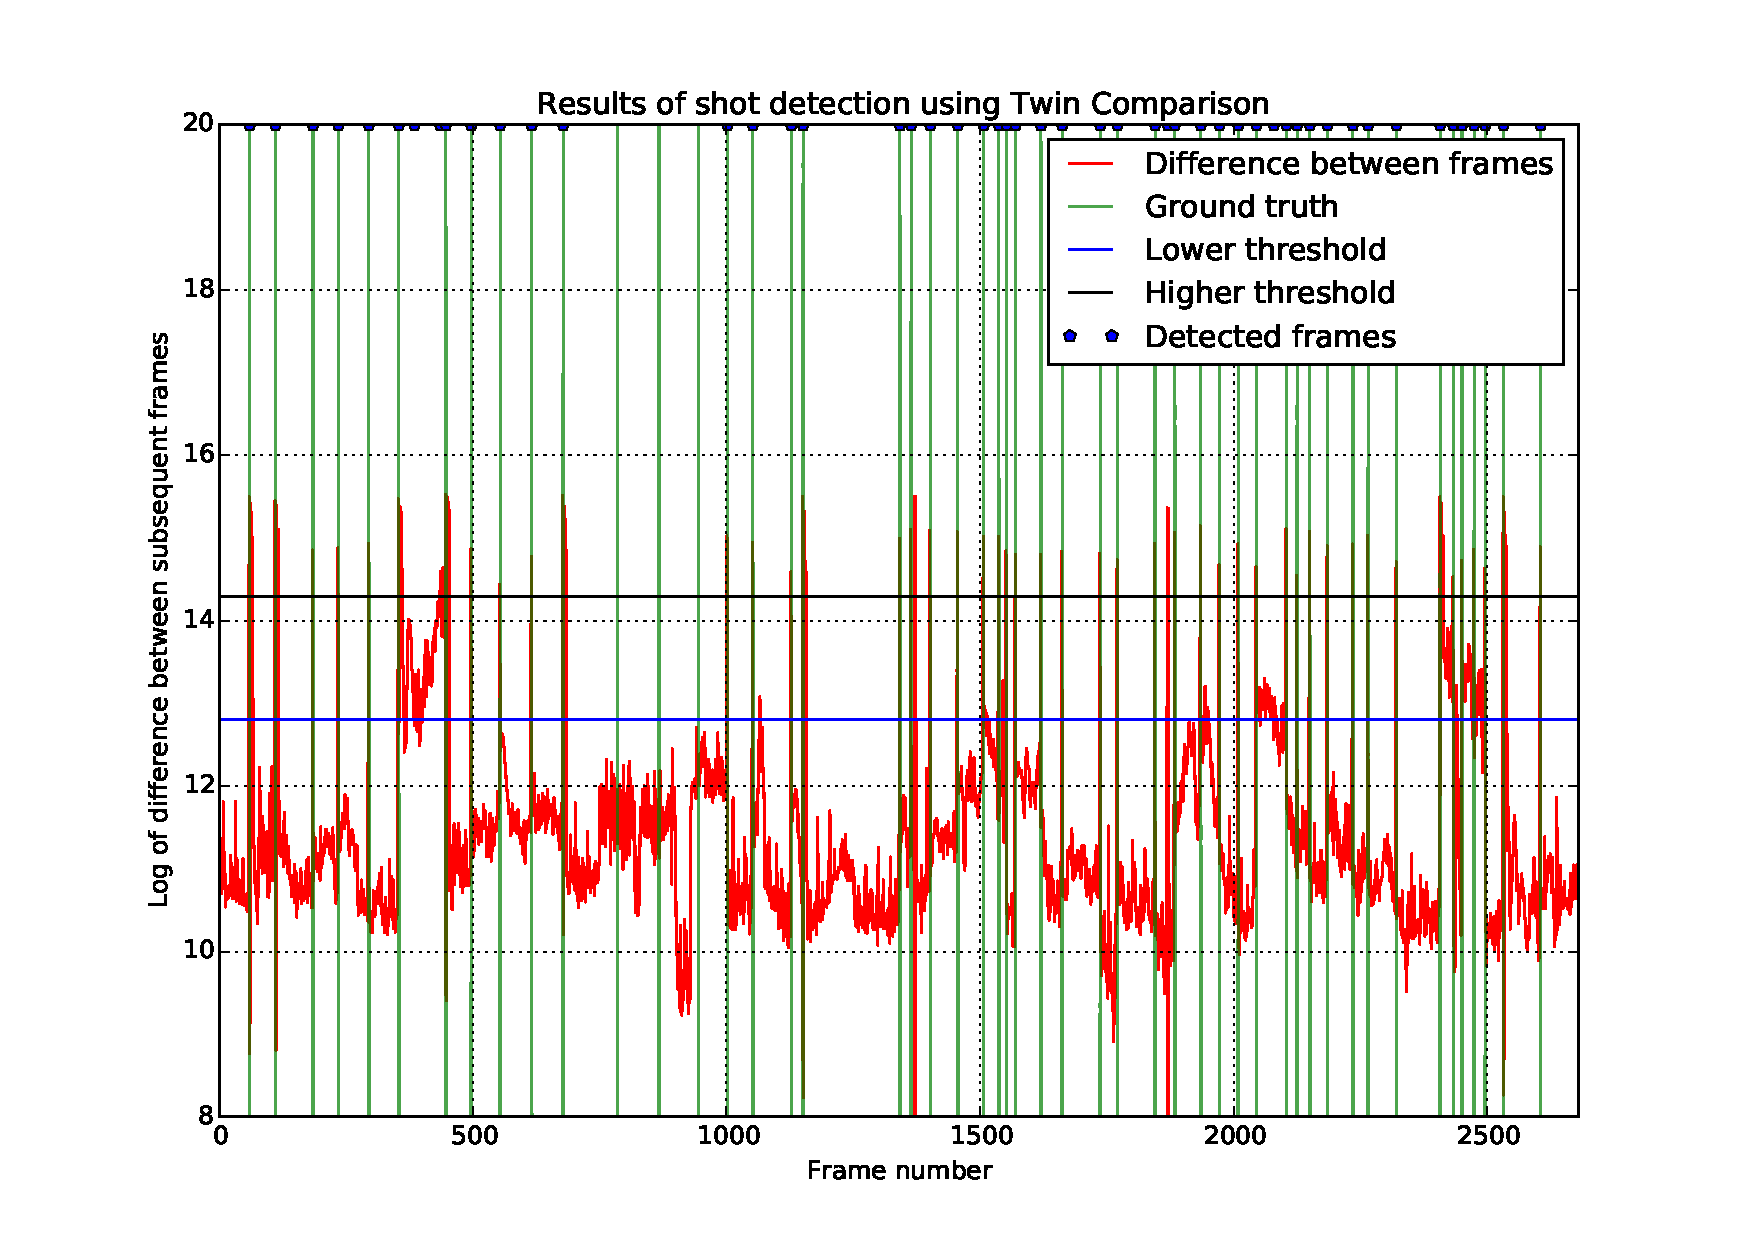
\includegraphics[page=1,angle=90,height=0.9\textheight,keepaspectratio]{figs/graph_entire_video}
  \caption{Results of Twin Comparison: entire video}
  \label{fig:entire}
\end{figure}

\newpage
\subsection{Twin Comparison graph: frame 0-800}
\label{app:zoom}

\begin{figure}[!ht]
  \centering
  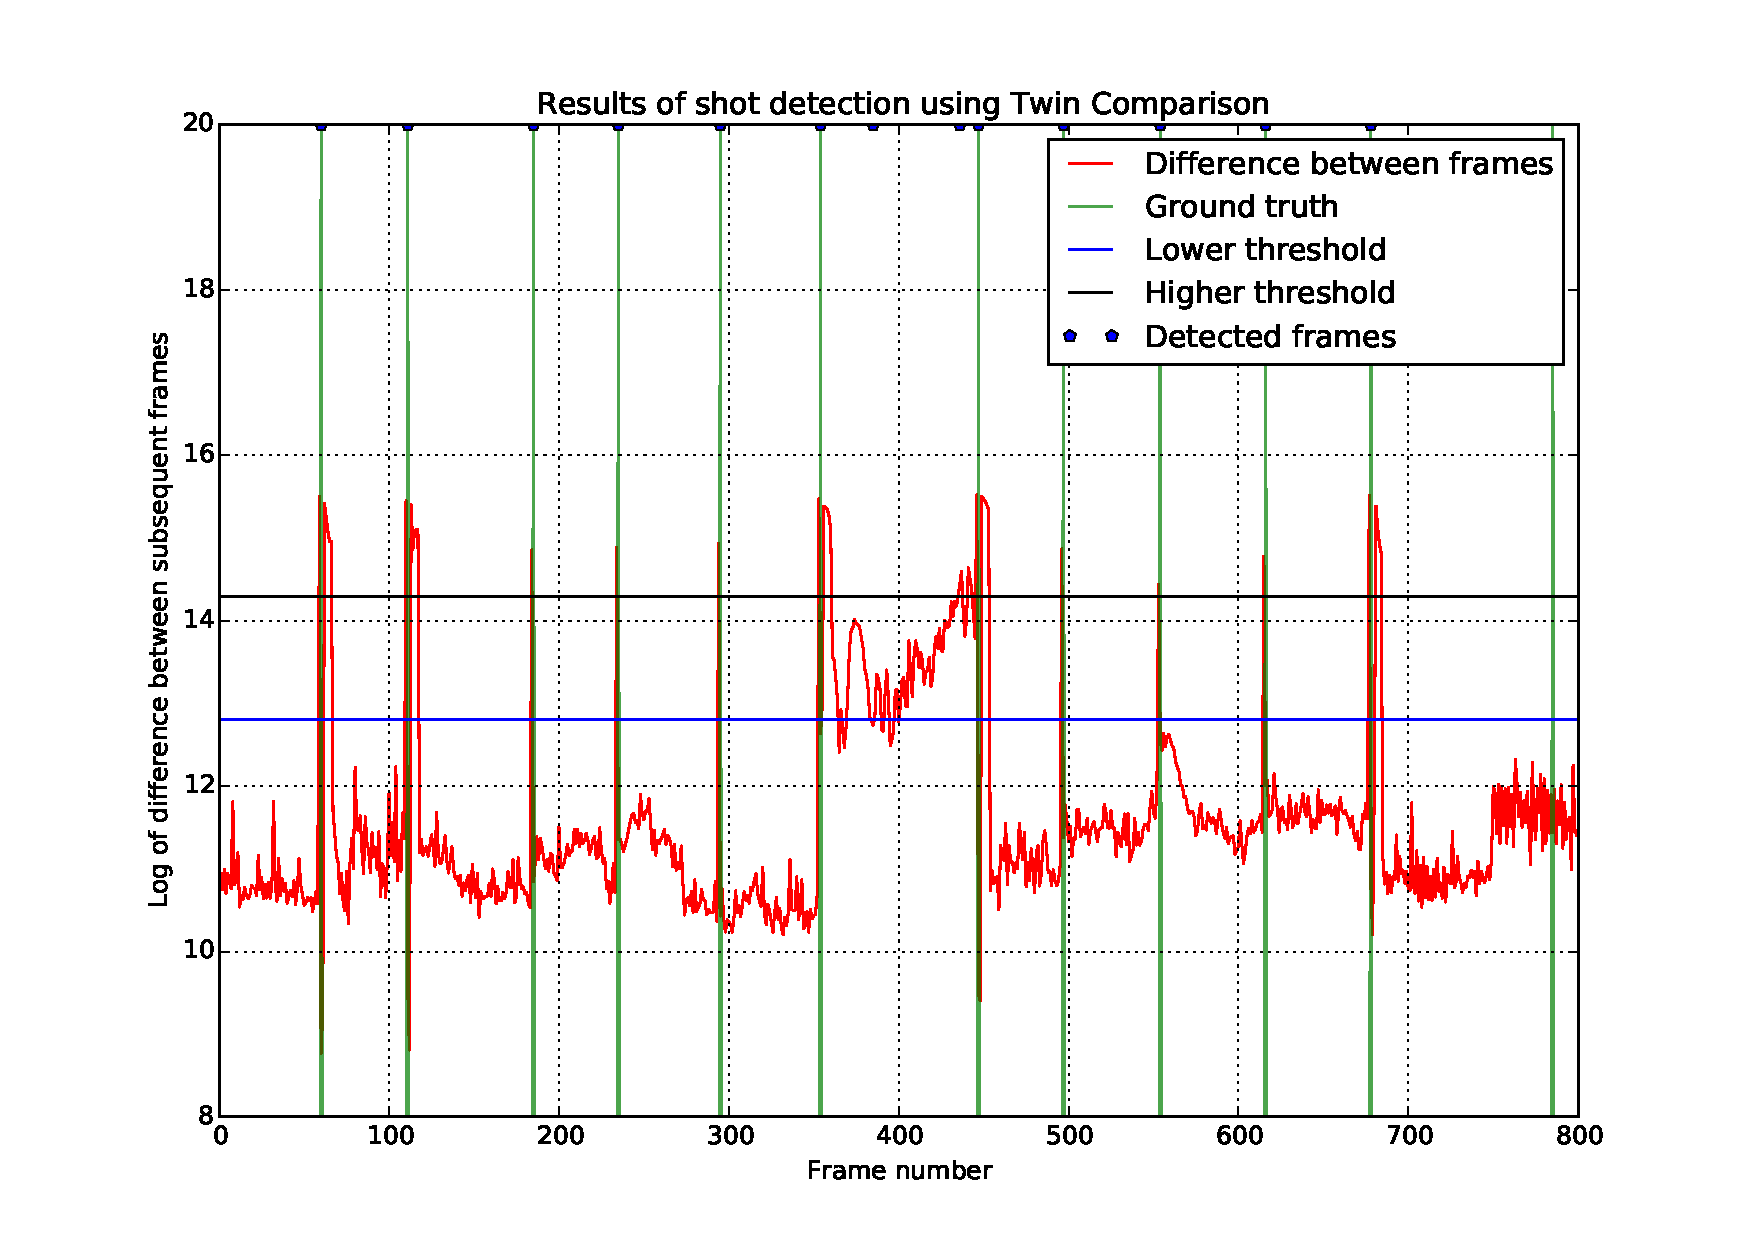
\includegraphics[page=1,angle=90,height=0.9\textheight,keepaspectratio]{figs/graph_zoom}
  \caption{Results of Twin Comparison: frame 0-800}
  \label{fig:zoom}
\end{figure}

\newpage

\subsection{Cause for false positives: Turbulent Sequences}
\label{app:turbulent}
\begin{figure}[ht]
  \centering
  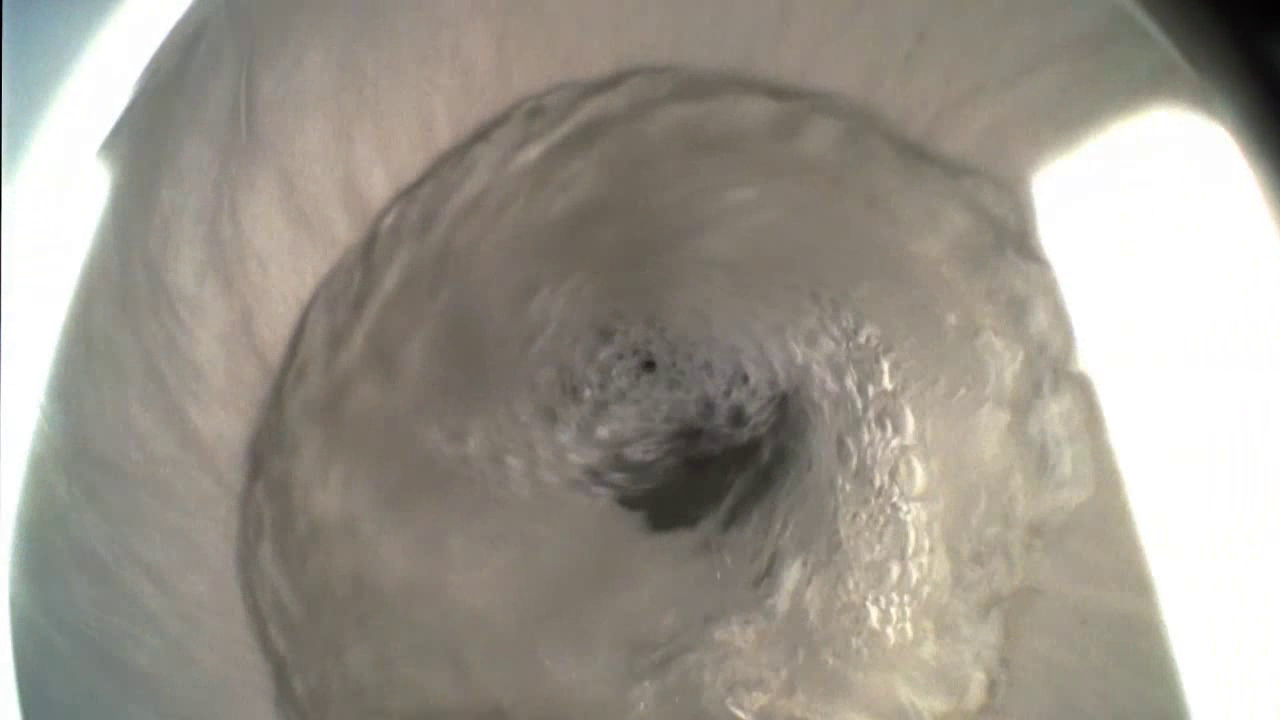
\includegraphics[width=.85\textwidth]{figs/turbulent}
  \caption{Turbulent sequences cause false positives}
  \label{fig:flush}
\end{figure}


\subsection{Cause for false negatives: Dissolves}
\label{app:dissolve}
\begin{figure}[ht]
  \centering
  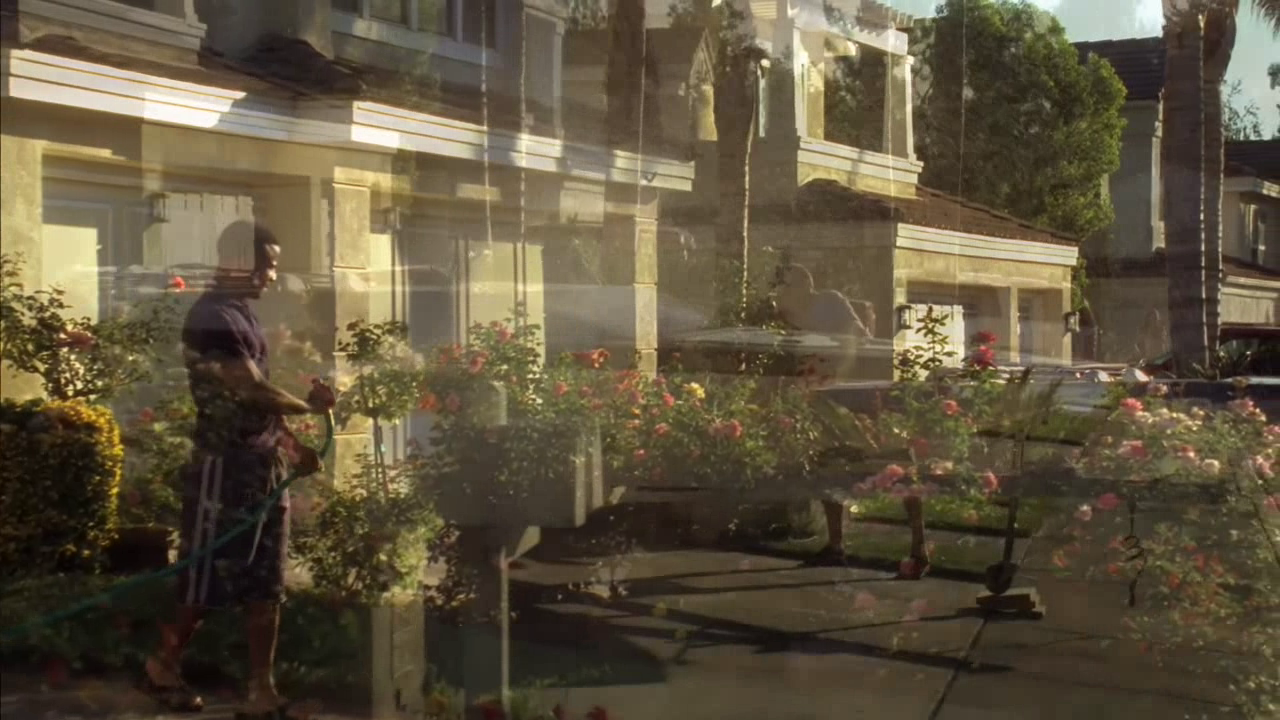
\includegraphics[width=.85\textwidth]{figs/dissolve}
  \caption{Dissolving transitions are hard to detect}
  \label{fig:dissolve}
\end{figure}

\newpage
\section{Q4}\label{app:q4}

\subsection{Setup}\label{q4:setup}
The used setup for all timings is: PC Configuration used for the measurements: 
\begin{enumerate}
\item Intel i5, 2 cores, 4 threads @2.5ghz 
\item 8GB dual-channel DDR3 @798Mhz RAM. 
\item GPU: Integrated Intel Hd graphics 4600 + NVIDIA GeForce GT 740M (2048MB dedicated RAM). 
\item The HD is a 700GB SATA-III 5400 RPM.
\end{enumerate}

\begin{table}[!ht]
\caption{Execution times (ms/frame) of different subsizes and search window sizes for the motion estimation.}
\label{execMotion}
\begin{tabular}{|l|l|l|l|l|l|l|}
\hline
\textbf{subSize (right)}\\ \textbf{searchWindow (below)}& \textbf{2} & \textbf{4} & \textbf{8} & \textbf{16} & \textbf{32} & \textbf{64} \\ \hline
\textbf{9}  & 49.36 & 41.33 & 46.78 & 42.26 & 42.63 & 47.64 \\ \hline
\textbf{11} & 48.60 & 40.33 & 44.05 & 42.05 & 42.31 & 40.08 \\ \hline
\textbf{15} & 51.07 & 43.10 & 44.30 & 43.23 & 40.51 & 39.36 \\ \hline
\textbf{19} & 87.80 & 85.20 & 80.47 & 82.22 & 77.30 & 80.21 \\ \hline
\end{tabular}
\end{table}

\begin{table}[!ht]
\caption{Execution times (ms/frame) of different bin counts for the global histogram method.}
\label{execGlobal}
\begin{tabular}{|l|l|l|l|l|l|l|l|l|l|l|}
\hline
\textbf{binCount}       & \textbf{25} & \textbf{50} & \textbf{75} & \textbf{100} & \textbf{125} & \textbf{150} & \textbf{175} & \textbf{200} & \textbf{225}  \\ \hline
\textbf{Execution time} & 2.36       & 2.62     & 2.38       & 2.62      & 2.83      & 2.37      & 2.32      & 2.32      & 2.35       \\ \hline
\end{tabular}
\end{table}

\begin{table}[!ht]
\caption{Execution times (ms/frame) of different region counts for the local histogram method.}
\label{execLocal}
\begin{tabular}{|l|l|l|l|l|l|l|l|l|l|l|}
\hline
\textbf{regionCount}    & \textbf{4} & \textbf{9} & \textbf{16} & \textbf{25} &\textbf{36}  & \textbf{49} & \textbf{64} & \textbf{81} \\ \hline
\textbf{Execution time} & 5.33    & 5.01     & 5.06     & 5.00     & 5.12     & 5.04     & 5.31     & 4.98     \\ \hline
\end{tabular}
\end{table}

\begin{table}[!ht]
\caption{Execution times (ms/frame) of different region counts for the Twin Comparison method.}
\label{twincomp}
\begin{tabular}{|l|l|l|l|l|l|l|l|l|l|l|}
\hline
\textbf{regionCount}    & \textbf{4} & \textbf{9} & \textbf{16} & \textbf{25} & \textbf{36} & \textbf{49} & \textbf{64} & \textbf{81} \\ \hline
\textbf{Execution time} & 5.20   & 5.22    & 5.04     & 5.22     & 5.17     & 5.34     & 5.43  & 5.75    \\ \hline
\end{tabular}
\end{table}

\section{Q5}\label{app:q5}
\subsection{Tables}

\begin{landscape}
\begin{table}[!ht]
\centering
\caption{ROC table part 1}
\label{ROCTable1}
\begin{tabular}{|l|l|l|l|l|l|l|}
\hline
\textbf{recall} & \textbf{pixelDistance} & \textbf{pixelFraction} & \textbf{motionDistance} & \textbf{motionFraction} & \textbf{globalFraction} & \textbf{localFraction} \\ \hline
\textbf{9}      &                        & 98                     & 90                      & 90                      &                         &                        \\ \hline
\textbf{23}     &                        & 98                     &                         &                         & 97                      &                        \\ \hline
\textbf{36}     & 92                     &                        &                         &                         &                         & 90                     \\ \hline
\textbf{50}     &                        &                        &                         &                         & 86                      &                        \\ \hline
\textbf{52}     &                        & 88                     &                         &                         &                         & 88                     \\ \hline
\textbf{57}     & 86                     &                        &                         &                         &                         &                        \\ \hline
\textbf{71}     & 71                     &                        &                         &                         &                         &                        \\ \hline
\textbf{76}     &                        &                        &                         &                         & 84                      &                        \\ \hline
\textbf{77}     &                        &                        &                         & 84                      &                         &                        \\ \hline
\textbf{78}     &                        &                        & 80                      &                         &                         &                        \\ \hline
\textbf{82}     & 29                     &                        &                         &                         &                         & 86                     \\ \hline
\textbf{83}     & 20                     & 51                     &                         &                         &                         &                        \\ \hline
\textbf{84}     &                        &                        & 76                      &                         & 63                      &                        \\ \hline
\textbf{88}     &                        &                        &                         & 43                      &                         &                        \\ \hline
\textbf{89}     &                        &                        &                         &                         &                         & 78                     \\ \hline
\textbf{90}     &                        &                        & 61                      &                         &                         &                        \\ \hline
\textbf{91}     &                        &                        & 55                      &                         & 41                      &                        \\ \hline
\textbf{93}     &                        &                        &                         &                         &                         & 51                     \\ \hline
\textbf{100}    &                        & 2                      &                         & 17                      & 2                       & 2                      \\ \hline
\end{tabular}
\end{table}
\end{landscape}


\begin{landscape}
\begin{table}[!ht]
\centering
\caption{ROC table part 2}
\label{ROCTable2}
\begin{tabular}{|l|l|l|l|l|}
\hline
\textbf{recall} & \textbf{TwinAlfa} & \textbf{TwinBeta} & \textbf{TwinGamma} & \textbf{TwinDelta} \\ \hline
\textbf{9}      &                   & 90                &                    &                    \\ \hline
\textbf{36}     &                   &                   &                    & 84                 \\ \hline
\textbf{43}     & 87                &                   &                    & 82                 \\ \hline
\textbf{56}     &                   & 87                &                    &                    \\ \hline
\textbf{58}     &                   &                   &                    & 78                 \\ \hline
\textbf{67}     &                   &                   &                    & 78                 \\ \hline
\textbf{72}     &                   &                   &                    & 76                 \\ \hline
\textbf{73}     & 86                &                   &                    &                    \\ \hline
\textbf{74}     &                   &                   &                    &                    \\ \hline
\textbf{75}     & 84                &                   & 82                 & 73                 \\ \hline
\textbf{76}     &                   & 83                & 84                 & 63                 \\ \hline
\textbf{77}     &                   &                   & 73                 &                    \\ \hline
\textbf{78}     &                   &                   & 73                 &                    \\ \hline
\textbf{82}     &                   & 67                &                    &                    \\ \hline
\textbf{84}     & 57                &                   &                    &                    \\ \hline
\textbf{87}     &                   &                   &                    & 37                 \\ \hline
\textbf{91}     & 22                &                   &                    &                    \\ \hline
\textbf{100}    &                   & 2                 &                    &                    \\ \hline
\end{tabular}
\end{table}
\end{landscape}
\clearpage

\subsection{ROC curves}
\subsubsection{Pixel}
\mijnfiguur{width=\textwidth}{rocPixel}{ROC curve for the pixel method (both distance and fraction variations)}
\subsubsection{Motion}
\mijnfiguur{width=\textwidth}{rocMotion}{ROC curve for the motion method (both distance and fraction variations)}
\clearpage
\subsubsection{Local and Global}
\mijnfiguur{width=0.9\textwidth}{rocGlobalLocal}{ROC curve for both the local and global histogram methods}
\subsubsection{Twin Comparison}
\mijnfiguur{width=0.9\textwidth}{rocTwin}{ROC curve for the twin comparison method (for alpha, beta, gamma and delta)}
\clearpage

\begin{landscape}
\begin{table}[h]
\caption{Precision, recall and F1 value for the different methods}
\label{ROCValues}
\begin{tabular}{|l|l|l|l|l|l|l|l|l|l|l|l|l|l|}
\hline
\textbf{Method}          & \textbf{Dist.} & \textbf{Fract.} & \textbf{Sub size} & \textbf{Window size} & \textbf{Bin cnt} & \textbf{Block cnt} & \textbf{A} & \textbf{B} & \textbf{C} & \textbf{D} & \textbf{Recall} & \textbf{precision} & \textbf{F1} \\ \hline
\textbf{pixel}           & 50                & 0.250             &                   &                      &                    &                      &            &            &            &            & 74              & 76                 & 74          \\ \hline
\textbf{Motion}          & 100               & 0.5               & 8                 & 11                   &                    &                      &            &            &            &            & 91              & 61                 & 73          \\ \hline
\textbf{Global}          &                   & 0.25              &                   &                      & 51                 &                      &            &            &            &            & 84              & 63                 & 72          \\ \hline
\textbf{Local}           &                   & 0.4               &                   &                      & 32                 & 9                    &            &            &            &            & 82              & 86                 & 84          \\ \hline
\textbf{Twin Comp.} &                   &                   &                   &                      & 32                 & 9                    & 1.5        & 0          & 1.0        & 2.0        & 82              & 86                 & 84          \\ \hline
\end{tabular}
\end{table}
\end{landscape}


\newpage
\section{Q6}\label{app:q6}
\begin{figure}[ht]
  \centering
  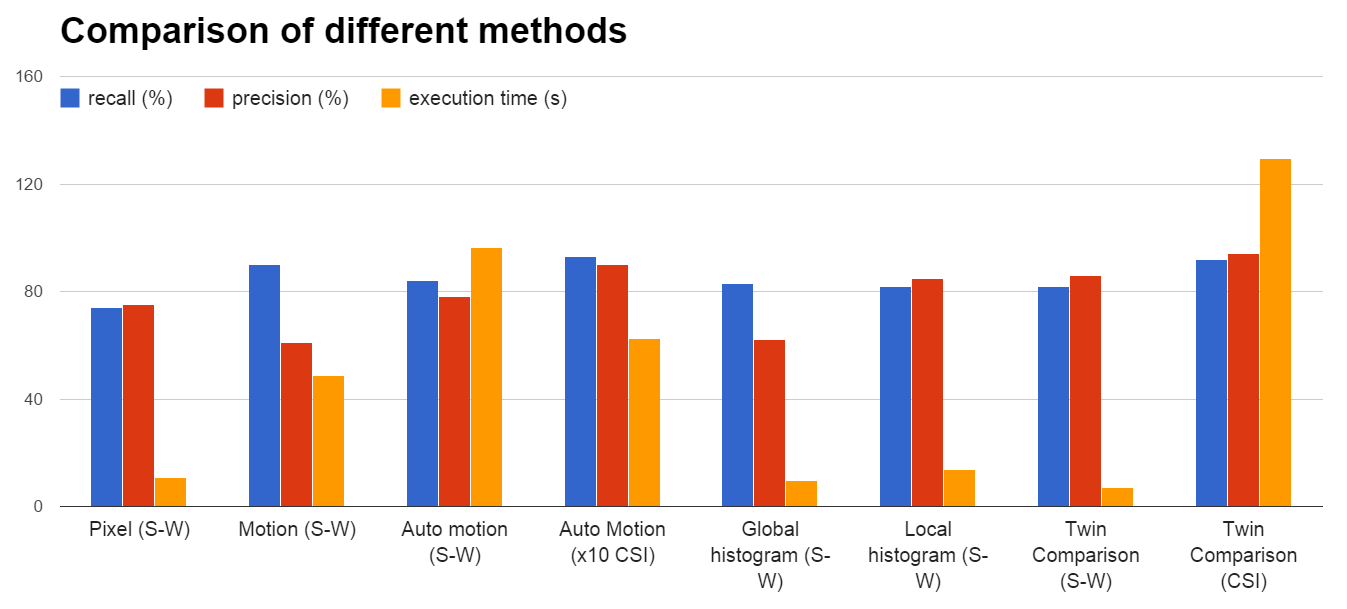
\includegraphics[page=1,angle=90,height=0.74\textheight,keepaspectratio]{grafiek}
  \caption{A comparison of the result}
  \label{grafiek}
\end{figure}

\end{appendices}